\chapter{Control}

Now that a functioning simulation environment is created and a inverse kinematics solver is created it is time to connect these to and create a controller to steer the robot manipulator. The initial thought is a multivariable control on top on single joint control. The multivariable control is done in Matlab, but it can be done in Python as well, but since the inverse kinematics problem is solved in MATLAB it is easiest to do the control in MATLAB. The multivariable control will use the joint positions and joint velocities to compute the desired joint torques which is sent to joint PID controllers which is handled by using ROS control package. The first thing to do is therefore to create the individual joint PID controllers. 
To create these controllers two new files are needed. A new launch file must be created. It is possible to just append the launch file, but to make everything more understandable and if the package is to be used on the real robot it is easier to make a new launch file that can be included in other launch files. The task of the control.launch file is to spawn a node which includes all of the five controllers. In \lstref{lst:launchControl} one can see the the code to spawn the controllers. It consists of two statements. The first is loading the parameters of the controllers from the YAML file. Then with the parameters loaded, a node is created and it makes the joint controller services that the wanted joint torques can be published to. 
\begin{lstlisting}[language=xml,caption={Spawns the controller node},label={lst:launchControl}]
<rosparam file="$(find five_dof_robotarm)/config/joints.yaml" command="load"/>

  <node name="controller_spawner" pkg="controller_manager" type="spawner" respawn="false"
	output="screen" ns="/five_dof_robotarm" args="joint_state_controller
    base_to_turntable_controller
    second_joint_controller
    third_joint_controller
    fourth_joint_controller
    fifth_joint_controller"/>
\end{lstlisting}
Below in \lstref{lst:matlabPubl} one can see how the publishers that will publish the desired joint torques calculated by the controller. 
\begin{lstlisting}[language=Matlab,caption={MATLAB code for creating the publishers.},label={lst:matlabPubl}]
pub1 = rospublisher('/five_dof_robotarm/base_to_turntable_controller/command','std_msgs/Float64');
pub2 = rospublisher('/five_dof_robotarm/second_joint_controller/command','std_msgs/Float64');
pub3 = rospublisher('/five_dof_robotarm/third_joint_controller/command','std_msgs/Float64');
pub4 = rospublisher('/five_dof_robotarm/fourth_joint_controller/command','std_msgs/Float64');
pub5 = rospublisher('/five_dof_robotarm/fifth_joint_controller/command','std_msgs/Float64');
\end{lstlisting}
%Pythoncode
\begin{comment}
\begin{lstlisting}[language=python,caption={Python code for creating the publishers.},label={lst:pythonPubl}]
#Define publishers for each joint position controller commands.
pub1 = rospy.Publisher('/five_dof_robotarm/first_joint_controller/command', Float64, queue_size=10)
pub2 = rospy.Publisher('/five_dof_robotarm/second_joint_controller/command', Float64, queue_size=10)
pub3 = rospy.Publisher('/five_dof_robotarm/third_joint_controller/command', Float64, queue_size=10)
pub4 = rospy.Publisher('/five_dof_robotarm/fourth_joint_controller/command', Float64, queue_size=10)
pub5 = rospy.Publisher('/five_dof_robotarm/fifth_joint_controller/command', Float64, queue_size=10)
\end{lstlisting}
\end{comment}


And how to publish the wanted torques is seen below in \lstref{lst:matlabPubs}. Here $u$ is the vector of the controller output. During the project it was also wanted to do the same in Matlab and the initial thought is the same and can be viewed in the appendix. 

\begin{lstlisting}[language=Matlab,caption={MATLAB code for publish wanted joint torques},label={lst:matlabPubs}]
    send(pub1,u(1))
    send(pub2,u(2))
    send(pub3,u(3))
    send(pub4,u(4))
    send(pub5,u(5))
\end{lstlisting}

\begin{comment}
\begin{lstlisting}[language=python,caption={Python code for publish wanted torques},label={lst:pythonPubs}]
pub1.publish(u[0,0])
pub2.publish(u[1,0])
pub3.publish(u[2,0])
pub4.publish(u[3,0])
pub5.publish(u[4,0])
\end{lstlisting}
\end{comment}


Another important functionallity to do control is to get the feedback from Gazebo with joint position and joint velocities. To do this a subscriber is needed. The subscriber can thought of as the opposite as the publisher. Instead of publishing values to a service, we instead want to listen to a service. 


\section{Control}

\subsection{PD controller with gravity compensation}

The controller that is going to be used is a simple PD controller with gravity compensation derived by \cite{spong}:
$$
    u=K_p\tilde{q} - K_d\dot{q} +g(q)
$$
 where $\tilde{q} = q_d - q$ and 
 \begin{align}\label{eq:gravity}
 g(q) = \frac{\partial P}{\partial q_k}
 \end{align}
 where the total potential energy for a n-link robot is $P = \sum^n_{i=1}P_i$. Where $P_i$ is the potential energy for each individual link. For this specific manipulator the center of mass is assumed in the geometric center of each link. In \cite{Siciliano} this controller is proven by using Lyapunov direct method to be globally asymptotically stable(GAS) as long as $K_d$ and $K_p$ is positive definite. It is important to keep in mind that if the online computing of $g(q)$ is not perfect, the statement of GAS does not hold. Based on the assumptions made, the controller can not guarantee GAS. 
 
 \subsection{Deriving the gravitational effect}
 The robot at hand starts and ends with twisting joints and only the three joints in the middle is rotational joints. This means that the potential energy is only dependent on $q_2$,$q_3$ and $q_4$ which makes calculating the potential energy a bit a easier. Because of this, the potential energy can be calculated by using a 2D sketch as shown in \figref{draw:pot-rob}.

\begin{figure}[htbp]
    \centering
    

%Thank you http://www.texample.net/tikz/examples/three-link-annotated/

\usetikzlibrary{patterns}

\newcommand{\nvar}[2]{%
    \newlength{#1}
    \setlength{#1}{#2}
}

% Define a few constants for drawing
\nvar{\dg}{0.3cm}
\def\dw{0.25}\def\dh{0.5}
\nvar{\ddx}{1.5cm}

% Define commands for links, joints and such
\def\link{\draw [double distance=1.5mm, very thick] (0,0)--}
\def\joint{%
    \filldraw [fill=white] (0,0) circle (5pt);
    \fill[black] circle (2pt);
}
\def\grip{%
    \draw[ultra thick](0cm,\dg)--(0cm,-\dg);
    \fill (0cm, 0.5\dg)+(0cm,1.5pt) -- +(0.6\dg,0cm) -- +(0pt,-1.5pt);
    \fill (0cm, -0.5\dg)+(0cm,1.5pt) -- +(0.6\dg,0cm) -- +(0pt,-1.5pt);
}
\def\robotbase{%
    \draw[rounded corners=8pt] (-\dw,-\dh)-- (-\dw, 0) --
        (0,\dh)--(\dw,0)--(\dw,-\dh);
    \draw (-0.5,-\dh)-- (0.5,-\dh);
    \fill[pattern=north east lines] (-0.5,-1) rectangle (0.5,-\dh);
}

% Draw an angle annotation
% Input:
%   #1 Angle
%   #2 Label
% Example:
%   \angann{30}{$\theta_1$}
\newcommand{\angann}[2]{%
    \begin{scope}[red]
    \draw [dashed, red] (0,0) -- (0pt,1.2\ddx);
    \draw [dashed, red] (0,0) -- (1.2\ddx,0pt);
    \draw [->, shorten >=3.5pt] ((0,\ddx) arc (90:#1:\ddx);
    % Unfortunately automatic node placement on an arc is not supported yet.
    % We therefore have to compute an appropriate coordinate ourselves.
    \node at (#1*2+2:\ddx-8pt) {#2};
    \end{scope}
}

% Draw line annotation
% Input:
%   #1 Line offset (optional)
%   #2 Line angle
%   #3 Line length
%   #5 Line label
% Example:
%   \lineann[1]{30}{2}{$L_1$}
\newcommand{\lineann}[4][0.5]{%
    \begin{scope}[rotate=#2, blue,inner sep=2pt]
        \draw[dashed, blue!40] (0,0) -- +(0,#1)
            node [coordinate, near end] (a) {};
        \draw[dashed, blue!40] (#3,0) -- +(0,#1)
            node [coordinate, near end] (b) {};
        \draw[|<->|] (a) -- node[fill=white] {#4} (b);
    \end{scope}
}

% Define the kinematic parameters of the three link manipulator.
\def\thetaone{30}
\def\Lone{2}
\def\thetatwo{30}
\def\Ltwo{1}
\def\thetathree{40}
\def\Lthree{1}


\begin{tikzpicture}
    %\robotbase
    \angann{\thetaone}{$q_2$}
    \lineann[-1]{\thetaone}{\Lone}{$L_2$}
    \link(\thetaone:\Lone);
    \joint
    \begin{scope}[shift=(\thetaone:\Lone), rotate=\thetaone]
        \angann{\thetatwo}{$q_3$}
        \lineann[-1.5]{\thetatwo}{\Ltwo}{$L_3$}
        \link(\thetatwo:\Ltwo);
        \joint
        \begin{scope}[shift=(\thetatwo:\Ltwo), rotate=\thetatwo]
            \angann{\thetathree}{$q_4$}
            \lineann[-1]{\thetathree}{\Lthree}{$L_4$}
            \draw [dashed, red,rotate=\thetathree] (0,0) -- (1.2\ddx,0pt);
            \link(\thetathree:\Lthree);
            \joint
            \begin{scope}[shift=(\thetathree:\Lthree), rotate=\thetathree]
                %\grip
            \end{scope}
        \end{scope}
    \end{scope}
\end{tikzpicture}

    \caption{Sketch of the robot the three middle joints of the robot}
    \label{draw:pot-rob}
\end{figure}
     
In \eqref{eq:potE} the potential energy is calculated for each link in the robot. 
 \begin{align}
    \begin{split}\label{eq:potE}
        P_1 &= m_1g\frac{L_1}{2}
        \\
        P_2 &= m_2g\left(L_1 + \frac{L_2}{2}\cos{(q_2)}\right)
        \\
        P_3 &= m_3g\left(L_1 +  L_2 \cos{(q_2)} + \frac{L_3}{2}\cos{(q_2 + q_3)} \right)
        \\
        P_4 &= m_4g\left(L_1 +  L_2 \cos{(q_2)} + L_3\cos{(q_2 + q_3)} + \frac{L_4}{2}\cos{(q_2+q_3+q_4)} \right)
        \\
        P_5 &=m_5g\left(L_1 +  L_2 \cos{(q_2)} + L_3\cos{(q_2 + q_3)} + \left(L_4 + \frac{L_5}{2} \right)\cos{(q_2+q_3+q_4)} \right)
        \\
        P &= P_1 + P_2 + P_3 + P_4 + P_5
    \end{split}   
 \end{align}    


 Where $L_4$ is the part up to the rotational joint. $L_5$ and $m_5$ is the rotational joint and the gripper together.  \\
 
 And then, to calculate individual gravity components equation \eqref{eq:gravity} is used on \eqref{eq:potE}:

 \begin{align*}
    g_1 &= 0
    \\
    g_2 &= \frac{\partial P}{\partial q_2} = 
    m_2g\frac{L_2}{2}\sin{(q_2)}+
    m_3g\left( L_2 \sin{(q_2)} + \frac{L_3}{2}\sin{(q_2+q_3)} \right)\\&+
    m_4g\left( L_2 \sin{(q_2)} + L_3\sin{(q_2 + q_3)} + \frac{L_4}{2}\sin{(q_2+q_3+q_4)} \right)\\&+
    m_5g\left( L_2 \sin{(q_2)} + L_3\sin{(q_2 + q_3)} + \left(L_4 + \frac{L_5}{2} \right)\sin{(q_2+q_3+q_4)} \right)
    \\
    g_3 &= \frac{\partial P}{\partial q_3} =
    m_3g\frac{L_3}{2}\sin{(q_2+q_3)} +
    m_4g\left( L_3\sin{(q_2 + q_3)} + \frac{L_4}{2}\sin{(q_2+q_3+q_4)} \right)\\&+
    m_5g\left(  L_3\sin{(q_2 + q_3)} + \left(L_4 + \frac{L_5}{2} \right)\sin{(q_2+q_3+q_4)} \right)
    \\
    g_4 &=\frac{\partial P}{\partial q_4} = 
    m_4g\frac{L_4}{2}\sin{(q_2+q_3+q_4)}+
    m_5g\left(L_4 + \frac{L_5}{2} \right)\sin{(q_2+q_3+q_4)}
    \\
    g_5 &= \frac{\partial P}{\partial q_5} = 0
    \\
    g(q) &= [g_1,g_2,g_3,g_4,g_5]^T
 \end{align*}
This is the gravity components that each joint will \textit{feel} from the other links and by adding this to a PD controller it will compensate for this disturbance. 

\section{Test of controller}
Now that a controller is in place it is time to test it. The first thing to test is the gravity compensation. One way to view the results is to watch the robot it is in a stationary state. The only input that are sent into the individual joint torque controllers should be the data computed only by the gravity compensation part. Some random desired joint angles is chosen and the following results can be viewed in \tabref{table:gravity}.\\\\
\begin{table}[htbp]
\centering
\caption{Test results of the precision of the gravity compensation}
\label{table:gravity}
    \begin{tabular}{l c c r}
        \toprule
        Joint  &  $g_i$ & $u_i$ & $u_i-g_i$\\
        \midrule
        1 & 0 & 0 & 0\\
        2 & -0.7720  & -0.7760  & -0.0040 \\
        3 &-0.4226 & -0.4191 & 0.0035 \\
        4 & -0.1870 &-0.1871 & -0.0001\\
        5 & 0 & 0 & 0\\
        \bottomrule
    \end{tabular}
\end{table}
One can see that the results are good. There is some error which means that the end effector will not be completely at its desired position. The biggest error is in the second joint and for this configuration $0.0022 rad = 0.1261 deg$\\\\
Now that we know that the gravity compensation is working we can start to test the controller. The gain matrices $K_p$ and $K_d$ are implemented as positive definite diagonal matrices.\\\\
\def\picsSiz{1.08}
\begin{figure*}[htbp]
    \centering
    \begin{subfigure}[htbp]{0.45\textwidth}
        \centering
        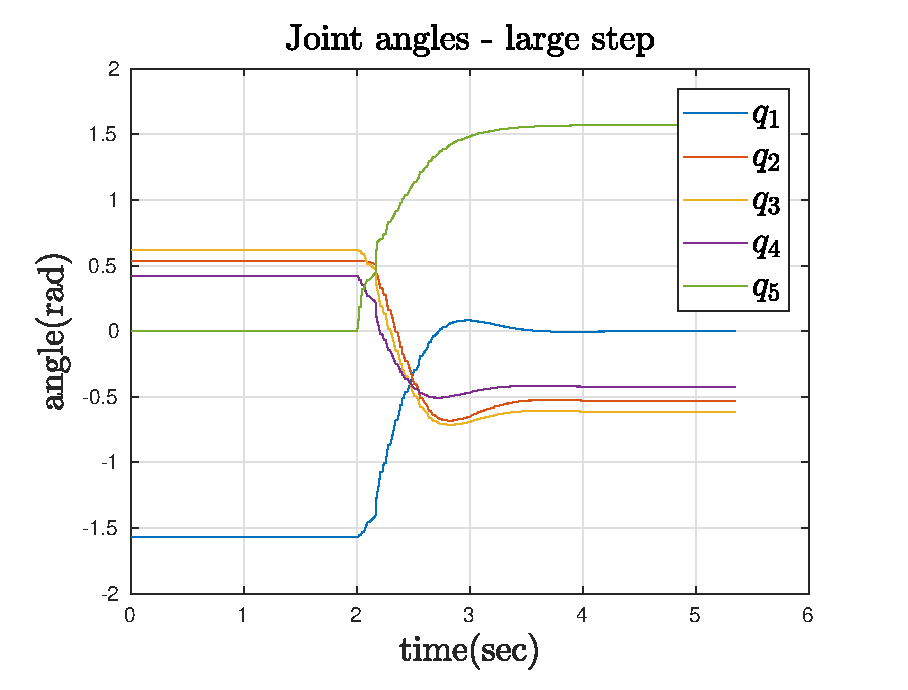
\includegraphics[width = \picsSiz\linewidth]{img/LSq.eps}
        \caption{ }
        \label{fig:LSq}
    \end{subfigure}
    ~ 
    \begin{subfigure}[htbp]{0.45\textwidth}
        \centering
        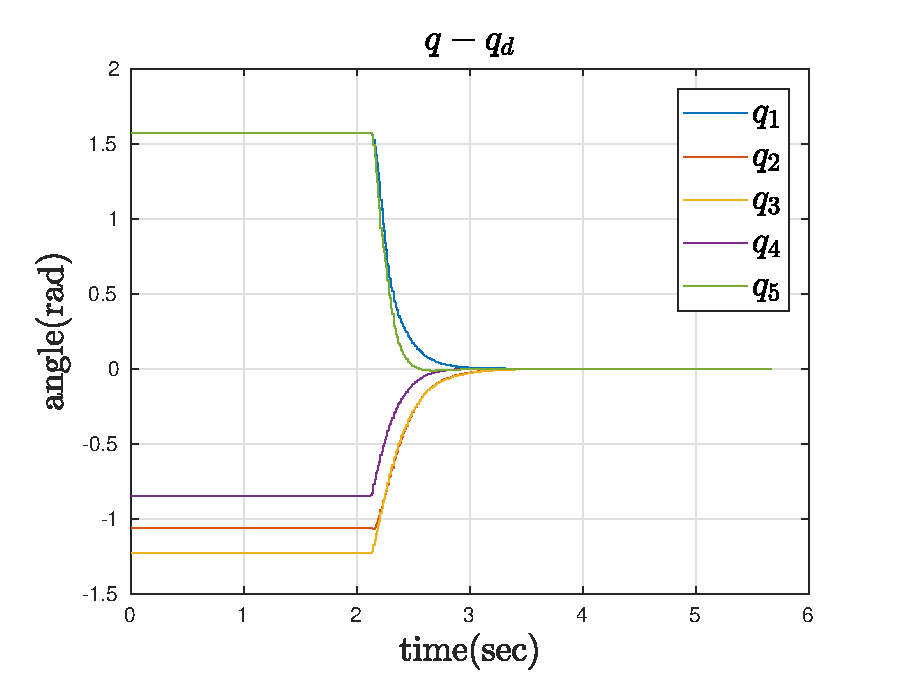
\includegraphics[width = \picsSiz\linewidth]{img/LSerror.eps}
        \caption{ }
    \end{subfigure}
    ~
    \centering
    \begin{subfigure}[htbp]{0.45\textwidth}
        \centering
        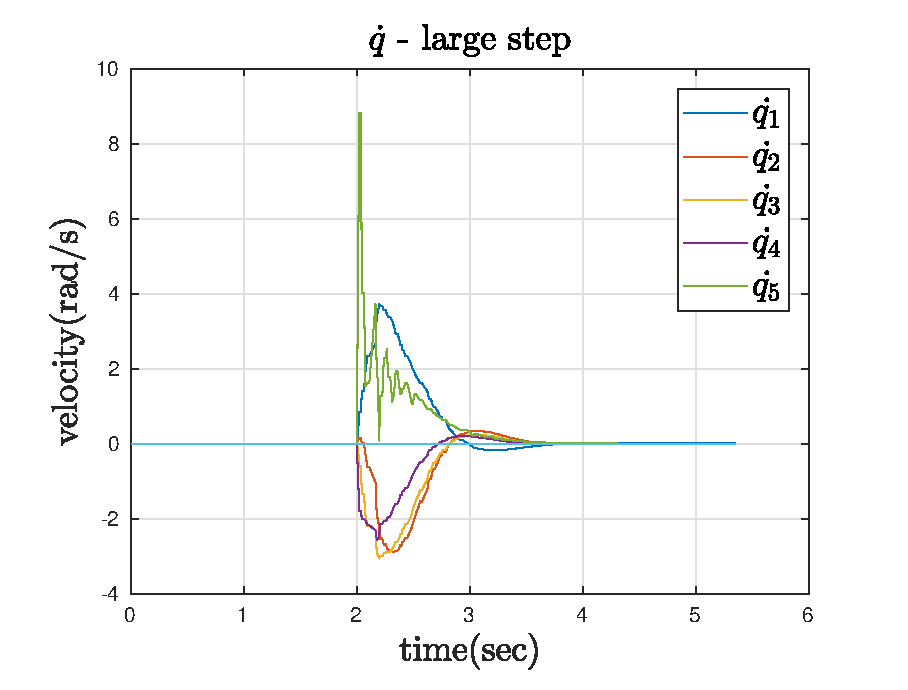
\includegraphics[width = \picsSiz\linewidth]{img/LSqdot.eps}
        \caption{ }
    \end{subfigure}
    ~ 
    \begin{subfigure}[htbp]{0.45\textwidth}
        \centering
        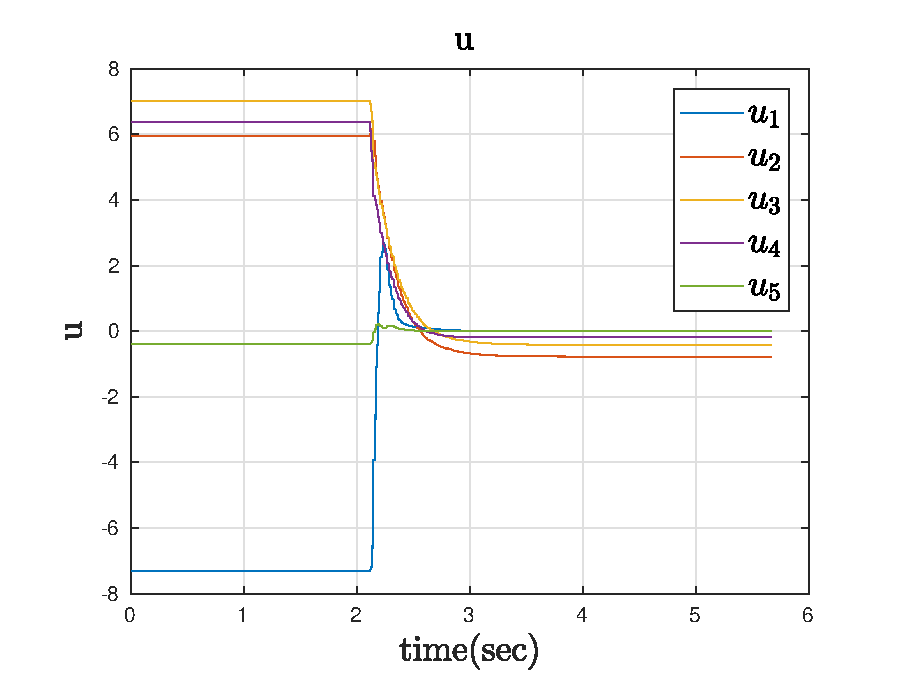
\includegraphics[width = \picsSiz\linewidth]{img/LSu.eps}
        \caption{ }
    \end{subfigure}
    ~
    \begin{subfigure}[htbp]{0.45\textwidth}
        \centering
        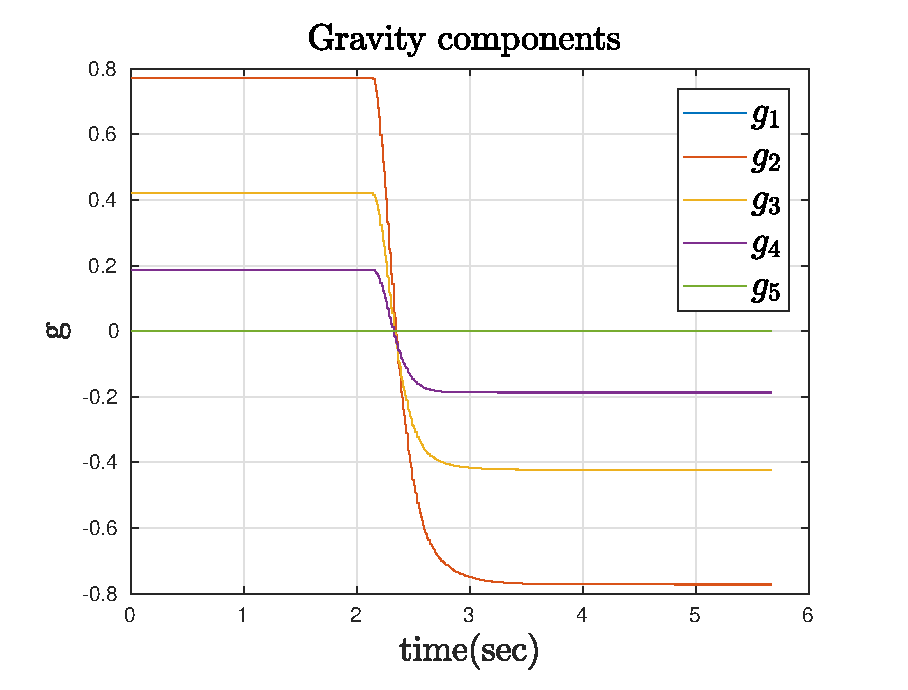
\includegraphics[width = \picsSiz\linewidth]{img/LSgrav.eps}
        \caption{ }
    \end{subfigure}
    \caption{Different plots of recorded data when a large step in desired joint angles is introduced}
    \label{fig:LS}
\end{figure*}
In \figref{fig:LS} data is plotted from a random configuration to a kind of inverse position such that every joint get to move. The step is rather large and because the intention of the robot arm is to do set point tracking some overshoot is therefore accepted for this case.  One thing that could be better is the joint velocity of last joint which seems a bit unstable. Additional tuning to try to avoid the bad input and joint velocity of the fifth joint results in slow convergence of the joint angle. Since the moments of inertia is very low and Gazebo handles low inertia very bad, this effect is assumed to be because of this and the when implementing this on the real robot it is expected that this effect will not be a problem. From \figref{fig:LSq} one can see $q_5$ converges rather smooth and the gains will be used for further testing. It may be worth to mention that when doing set point tracking the steps are not be this large and the gains can be altered for better performance.  \\\\






\section{Trajectory planning}
\subsection{Point to point tracking}
The main objective is to follow a path so it is desirable to test the controller for a path as well. The \figref{fig:pathTS} shows how each joint manages to follow the desired path shown in \figref{fig:IKcom}. One can see that the robot lags behind the desired path. This path is only time dependent so it changes without respect to if the robot arm has managed to get the desired position or not.\\\\
\def\picsSiz{1.08}
\begin{figure*}[htbp]
    \centering
    \begin{subfigure}[htbp]{0.45\textwidth}
        \centering
        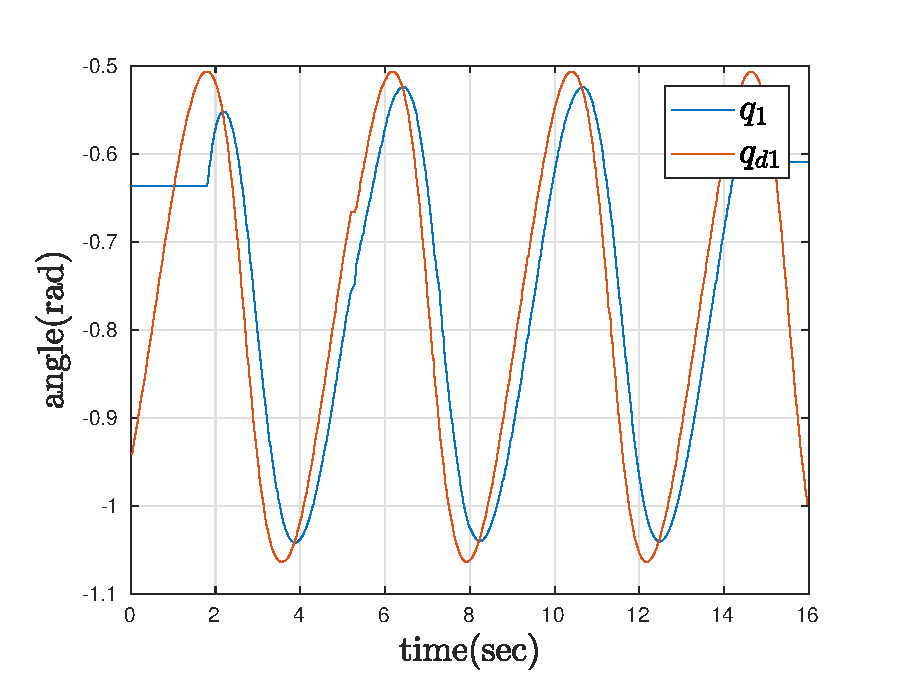
\includegraphics[width = \picsSiz\linewidth]{img/pathF1.eps}
        \caption{}
    \end{subfigure}
    ~ 
    \begin{subfigure}[htbp]{0.45\textwidth}
        \centering
        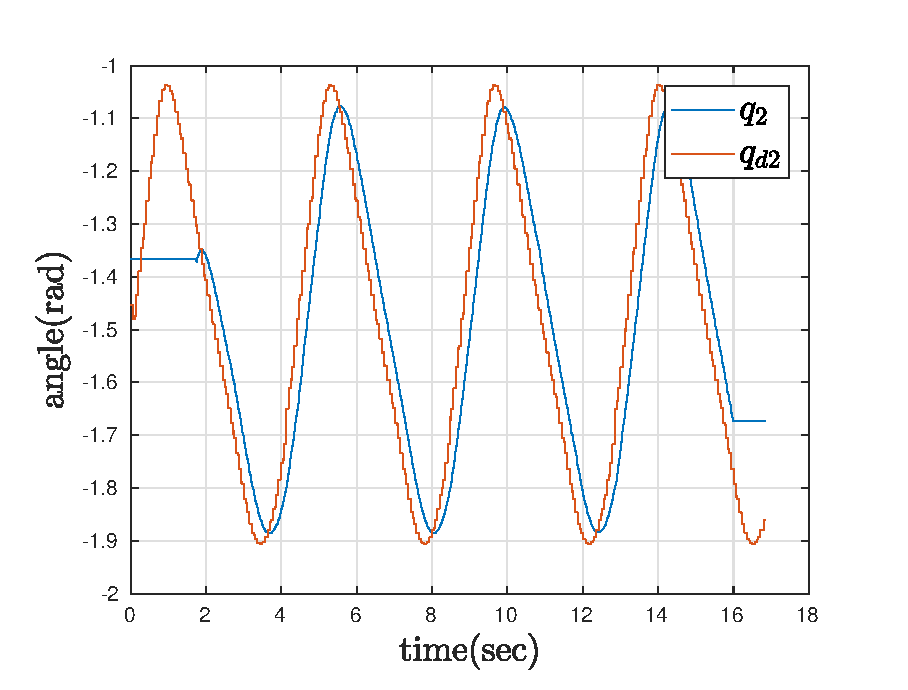
\includegraphics[width = \picsSiz\linewidth]{img/pathF2.eps}
        \caption{}
    \end{subfigure}
    ~
    \centering
    \begin{subfigure}[htbp]{0.45\textwidth}
        \centering
        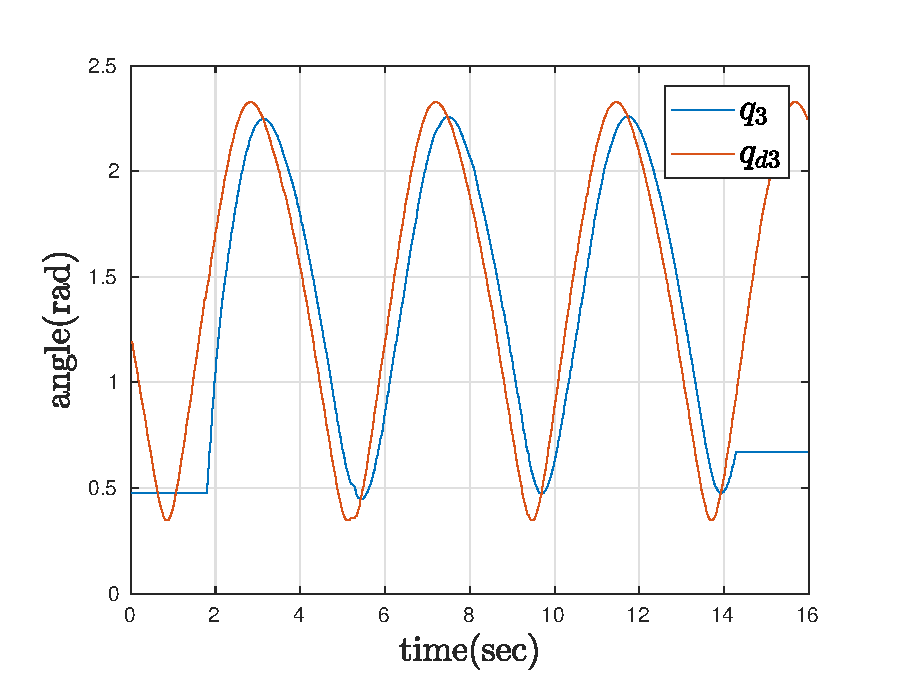
\includegraphics[width = \picsSiz\linewidth]{img/pathF3.eps}
        \caption{}
    \end{subfigure}
    ~ 
    \begin{subfigure}[htbp]{0.45\textwidth}
        \centering
        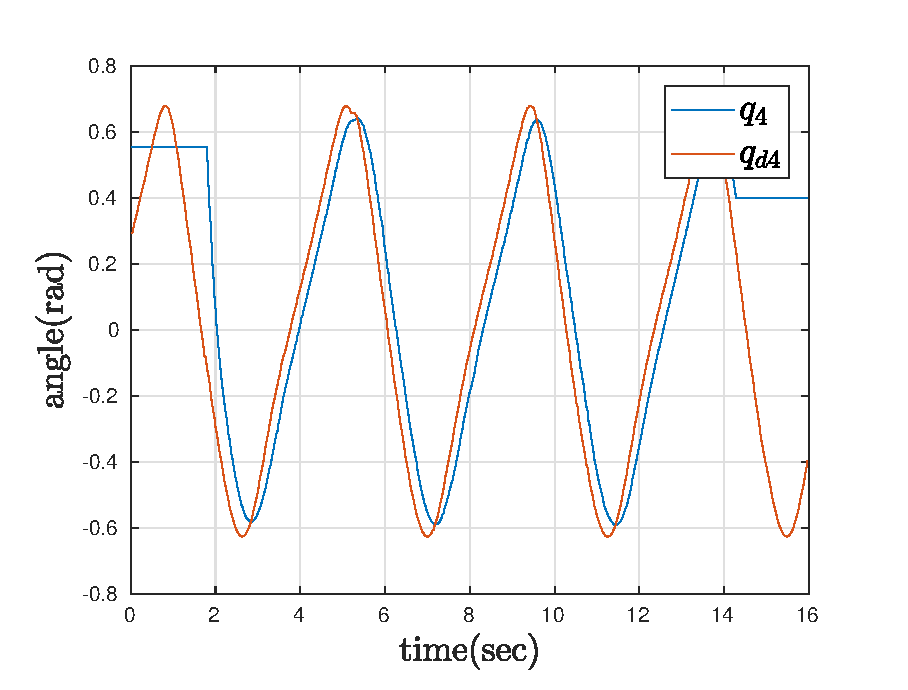
\includegraphics[width = \picsSiz\linewidth]{img/pathF4.eps}
        \caption{}
    \end{subfigure}
    ~
    \begin{subfigure}[htbp]{0.45\textwidth}
        \centering
        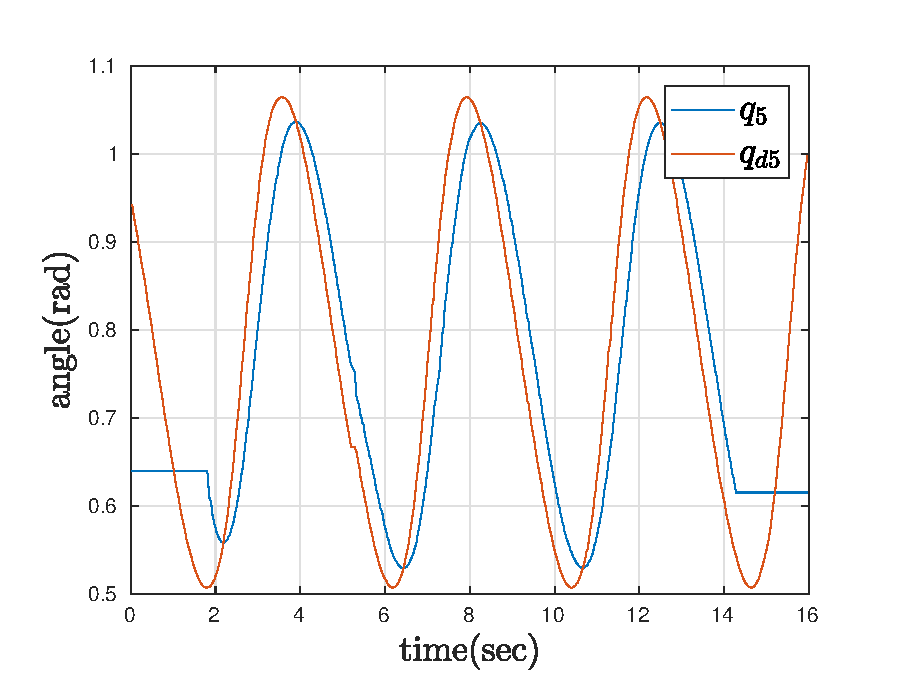
\includegraphics[width = \picsSiz\linewidth]{img/pathF5.eps}
        \caption{}
    \end{subfigure}
    \caption{Path following}
    \label{fig:pathTS}
\end{figure*}
The only information the robot gets is the point it is supposed to get to. It is therefore wanted to pass it some more information about the path. \cite{Siciliano} gives a method to use the slope of the trajectory to find the joint velocity in the trajectory
\begin{align*}
    \dot{q}_i = 
    \begin{cases}
    0\hphantom{ \frac{1}{2}(v_i+v_{i+1})}\;\;sgn(v_k)\ne sgn(v_{i+1})\\
    \frac{1}{2}(v_i+v_{i+1}) \quad  sgn(v_i)= sgn(v_{i+1})
    \end{cases}
\end{align*}
where $v_i = \frac{q_i-q_{i-1}}{t_i-t_{i-1}}$ and when you get to the last point $N$ the joint velocity $q_N$ should be zero. Since the error between the executed trajectory and the desired trajectory can be seen as a time delay one can also add the next points as a reference:
\begin{align*}
    \tilde{q} = q_{d_i}-q + \frac{q_{d_{i+1}}-q }{2}+\frac{q_{d_{i+2}}-q }{2}
\end{align*}
The results are given in \figref{fig:pathTSff}. One can see that the error is almost gone. 



\def\picsSiz{1.08}
\begin{figure*}[htbp]
    \centering
    \begin{subfigure}[htbp]{0.45\textwidth}
        \centering
        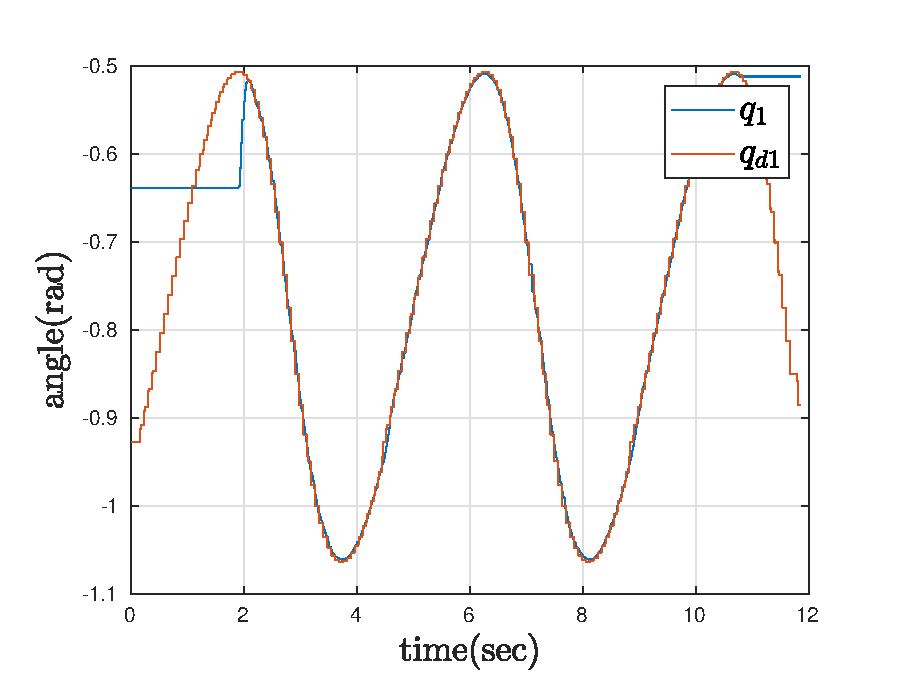
\includegraphics[width = \picsSiz\linewidth]{img/pathF1ff.eps}
        \caption{ }
    \end{subfigure}
    ~ 
    \begin{subfigure}[htbp]{0.45\textwidth}
        \centering
        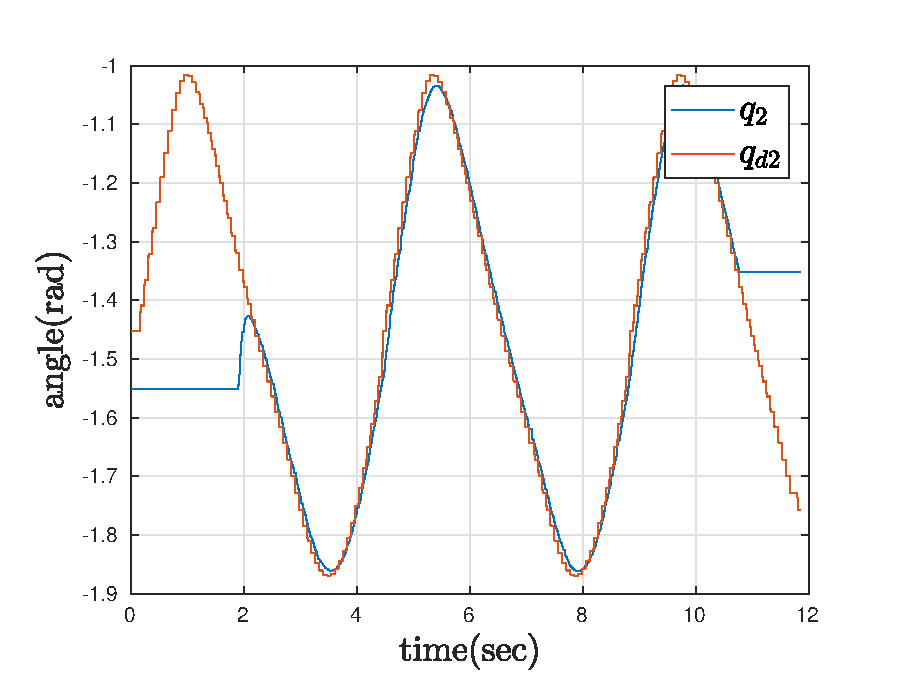
\includegraphics[width = \picsSiz\linewidth]{img/pathF2ff.eps}
        \caption{ }
    \end{subfigure}
    ~
    \centering
    \begin{subfigure}[htbp]{0.45\textwidth}
        \centering
        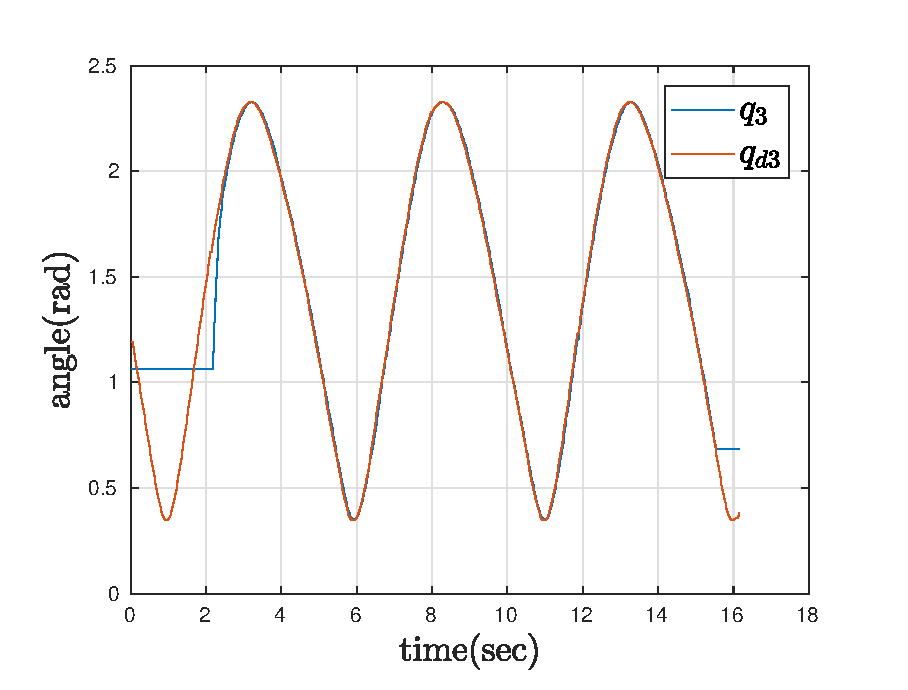
\includegraphics[width = \picsSiz\linewidth]{img/pathF3ff.eps}
        \caption{ }
    \end{subfigure}
    ~ 
    \begin{subfigure}[htbp]{0.45\textwidth}
        \centering
        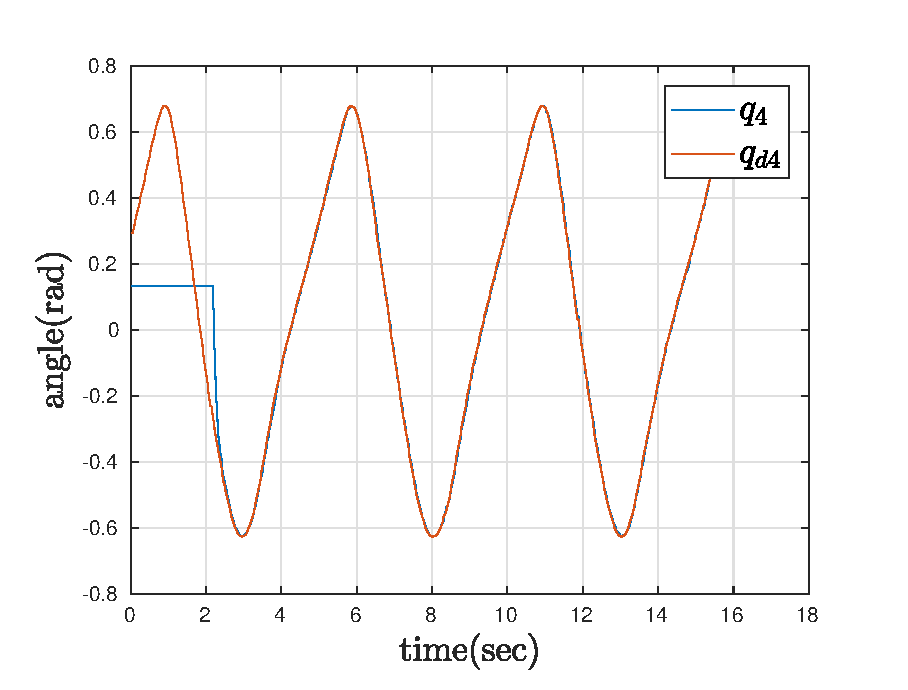
\includegraphics[width = \picsSiz\linewidth]{img/pathF4ff.eps}
        \caption{ }
    \end{subfigure}
    ~
    \begin{subfigure}[htbp]{0.45\textwidth}
        \centering
        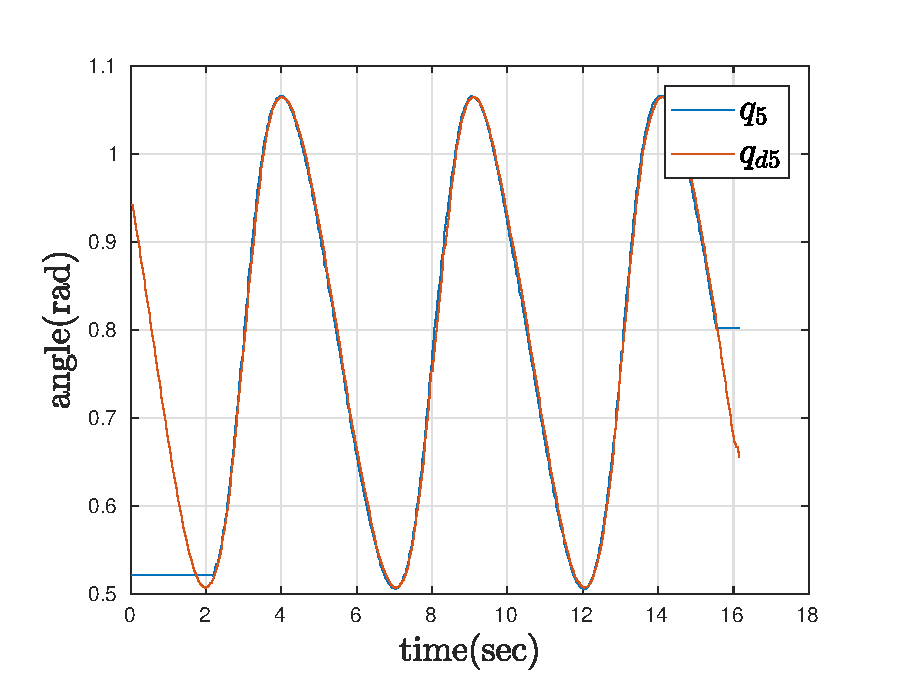
\includegraphics[width = \picsSiz\linewidth]{img/pathF5ff.eps}
        \caption{ }
    \end{subfigure}
    \caption{Path following with trajectory planner}
    \label{fig:pathTSff}
\end{figure*}


\section{Motion planning}
Until now we have just used a predefined path that has been made to test the different aspects of the manipulator. If it is wanted to go to one point to another it can be solved by creating a spline between these two points and do path following\cite{Spline}\cite{MatlabSpline}. The task in not so easy if there are obstacles present. We then need to find a set of points such that the obstacle is avoided. One algoritgm for solving this is the \textit{rapidly-exploring random tree (RRT)} which gives good results without any parameter tuning\cite{Lavalle}. 
\subsection{Rapidly exploring Random Tree (RRT)}
The RRT algorithm is creating a space-filling tree and in our case it can be used with obstacles in the search space such that the obstacle will be an illegal object where the three cannot expand and thus using shortest path algorithm to find a path trough the tree such that we get to the desired point and avoiding the obstacle. In \figref{fig:rrt2dex} an example is given of the algorithm. An obstacle ha been placed in the search space and the wanted point is behind the obstacle relative to the origin \cite{rrt}.
\begin{figure}[htbp]
  \centering
  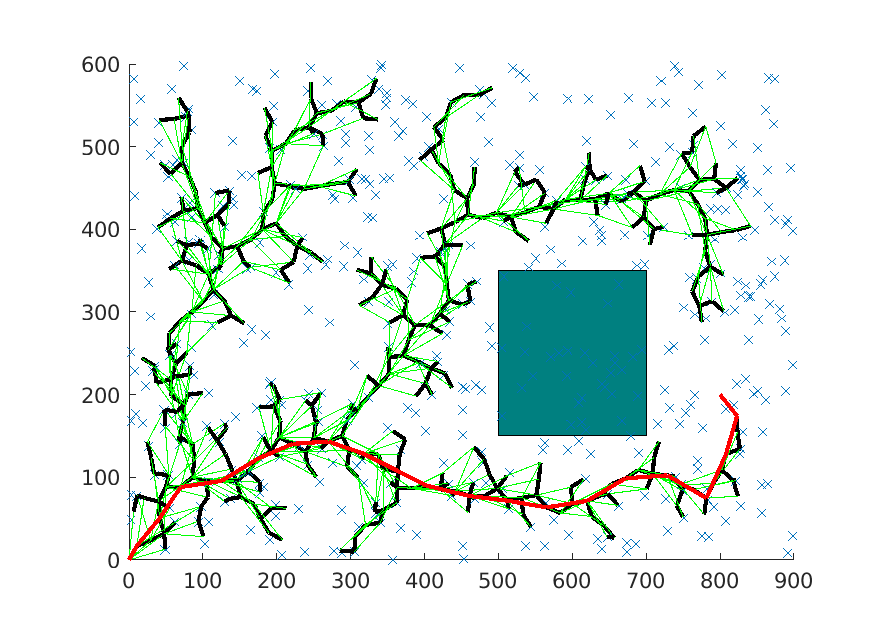
\includegraphics[width=.9\textwidth]{img/rrt2dex.eps}
  \caption{2D example of the RRT algoritm}
  \label{fig:rrt2dex}
\end{figure}
The next step is to expand this to a 3D example and do the same there. The toolbox provided by \cite{rrt} does include 3D RRT but not with obstacle avoidance unfortunately. The source code is given though, which mean it can be augmented into covering 3D obstacle avoidance. In \figref{fig:rrt3dex} the result of RRT in 3D space is presented. The red line is the lines between the nodes in the tree which shows a path to the desired point. 

\def\picsSiz{1.08}
\begin{figure*}[htbp]
    \centering
    \begin{subfigure}[htbp]{0.45\textwidth}
        \centering
        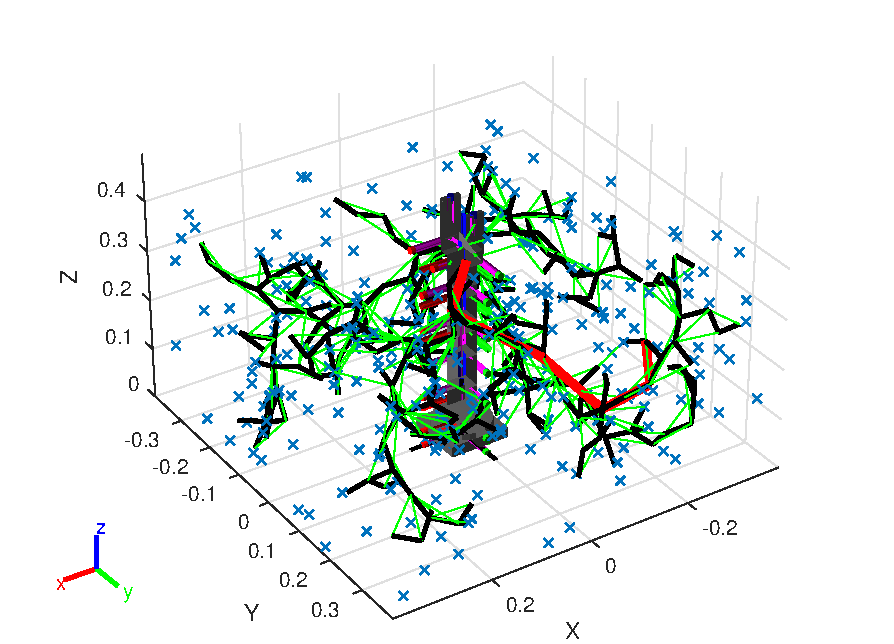
\includegraphics[width = \picsSiz\linewidth]{img/rrt3dex.eps}
        \caption{Result of the RRT algorithm}
        \label{fig:rrt3dex}
    \end{subfigure}
    ~ 
    \begin{subfigure}[htbp]{0.45\textwidth}
        \centering
        \includegraphics[width = \picsSiz\linewidth]{img/rrtSpline.eps}
        \caption{A spline is found based on the results}
    \end{subfigure}
    \caption{3D example of the RRT algoritm}
    \label{fig:rrtsuper}
\end{figure*}
 As one can see in \figref{fig:rrt3dex} there are some green lines which is shortcuts between nodes. These can help to choose less nodes if that is wanted. These green lines need to be checked for collision as well. 
 
 \subsubsection{Obstacle avoidance}
 To add obstacle avoidance one have to check if the straight line between the new node and its parent node does not intersect.